\documentclass[authordate,empirical, issue]{jote-new-article}
\addbibresource{bibliography.bib}

\jotetitle{Challenges of Using Signaling Data From Telecom Network in Non-Urban Areas}
\keywordsabstract{avalanche, risk, signaling data, telecom, non-urban areas}
\abstracttext{Outdoor recreation continues to increase in popularity. In Norway, several avalanche fatalities are recorded every year, but the accurate calculation of a fatal accident rate is impossible without knowing how many people are exposed. We attempted to employ signaling data from telecom networks to enumerate backcountry travelers in avalanche terrain. Each signaling data event contains information about which coverage area the phone is connected to and a timestamp. There is no triangulation, making it impossible to know whether the associated phone is moving or stationary within the coverage area. Hence, it is easier to track the phone's movement through different coverage areas. We utilize this by enumerating the number of people with phones traveling to avalanche-prone terrain for the 2019-2020 winter season. We estimated that 13,666 phones were in avalanche terrain during the season, ranging from 0 to 118 phones per day with an average of 75 phones per day. We correlated the number of phones per day against amount of daylight (\emph{R}\textsuperscript{2}=0.186, \emph{p} < 0.01), weekends and holidays (\emph{R}\textsuperscript{2}=0.073, \emph{p} < 0.01), and number of bulletin views (\emph{R}\textsuperscript{2}=0.045, \emph{p} < 0.01). Unfortunately, the validation revealed discrepancies between the estimated positions in the mobile network and the true reference positions as collected with a GPS. We attribute this to the algorithm being designed to measure urban mobility and the long distance between the base transceiver stations in mountainous areas. This lack of coherence between the signaling data and GPS records for rural areas in Norway has implication for the utility of signaling data outside of urban regions.}
\runningauthor{Toft et al.}
\jname{Journal of Trial \& Error}
\jyear{2023}
\paperdoi{10.36850/e14}
\paperreceived{July 8, 2022}
\author[1,2]{Håvard Boutera Toft\orcid{0000-0003-1748-6329}}
\affil[1]{Norwegian Water Resources and Energy Directorate}
\affil[2]{UiT The Arctic University of Norway}
\affil[3]{Telia Company}
\affil[4]{Antarctica New Zealand}
\corremail{\href{mailto:htla@nve.no}{htla@nve.no}}
\corraddress{Norwegian Water Resources and Energy Directorate}
\runningauthor{Toft et al.}
\author[3]{Alexey Sirotkin\orcid{0000-0002-4024-7943}}
\author[1,2]{Markus Landrø\orcid{0000-0001-5961-4697}}
\author[1,2]{\mbox{Rune Verpe Engeset\orcid{0000-0003-2608-2895}}}
\author[4,2]{Jordy Hendrikx\orcid{0000-0001-6194-3596}}
\paperaccepted{December 14, 2022}
\paperpublished{May 3, 2023}
\paperpublisheddate{2023-05-03}
\jwebsite{https://journal.trialanderror.org}


\jvolume{3}
\jissue{1}
\paperissued{December 18, 2023}
\jpages{72--84}

\begin{filecontents}{bibliography.bib}
	@article{Birkeland2017,
    title       = {In Response to Avalanche Fatalities in the United States by Jekich et al},
    author      = {Birkeland, K. W. and Greene, E. M. and Logan, S.},
    number      = {4},
    volume      = {28},
    url         = {https://doi.org/10.1016/j.wem.2017.06.009},
    doi         = {10.1016/j.wem.2017.06.009},
    publisher   = {Elsevier Ltd},
    date        = {2017},
    pages       = {380–382},
    journal     = {Wilderness and Environmental Medicine}
}


@book{Buhler2016,
    title       = {Using crowdsourced data to understand terrain usage patterns of backcountry recreational users},
    author      = {Buhler, R. and Floyer, J.},
    publisher   = {International Snow Science Workshop},
    place       = {Breckenridge, USA},
    date        = {2016}
}


@article{Engeset2018,
    title       = {Communicating public avalanche warnings – what works?},
    author      = {Engeset, R.v and Pfuhl, G. and Landrø, M. and Mannberg, A. and Hetland, A.},
    volume      = {18},
    url         = {https://doi.org/https://doi.org/10.5194/nhess-18-2537-2018},
    doi         = {10.5194/nhess-18-2537-2018},
    date        = {2018},
    pages       = {2537–2559},
    journal     = {Natural Hazards and Earth System Science}
}


@article{Ebert2019,
    title       = {Bayesian reasoning in avalanche terrain: a theoretical investigation},
    author      = {Ebert, P. A.},
    number      = {1},
    volume      = {19},
    url         = {https://doi.org/10.1080/14729679.2018.1508356},
    doi         = {10.1080/14729679.2018.1508356},
    date        = {2019},
    pages       = {84–95},
    journal     = {Journal of Adventure Education and Outdoor Learning}
}


@book{Francisco2018,
    title       = {Exploring the potential of mobile phone data (call detail records) to track and analyze backcountry skiers’ dynamics in avalanche terrain},
    author      = {Francisco, G. and Apodaka, J. and Travesset-Baro, O. and Vilella, M. and Margalef, A. and Pons, M.},
    publisher   = {International Snow Science Workshop},
    place       = {Innsbruck, Austria},
    date        = {2018}
}


@article{González2008,
    title       = {Understanding individual human mobility patterns},
    author      = {González, M. C. and Hidalgo, C. A. and Barabási, A.-L.},
    number      = {7196},
    volume      = {453},
    url         = {https://doi.org/10.1038/nature06958},
    doi         = {10.1038/nature06958},
    date        = {2008},
    pages       = {779–782},
    journal     = {Nature}
}


@book{Hendrikx2014,
    title       = {Using global crowd-sourced data to understand travel behavior in avalanche terrain},
    author      = {Hendrikx, J. and Johnson, J.},
    publisher   = {International Snow Science Workshop},
    place       = {Banff, Canada},
    date        = {2014},
    pages       = {224–227}
}


@article{Hendrikx2016,
    title       = {Using {GPS} tracking to explore terrain preferences of heli-ski guides},
    author      = {Hendrikx, Jordy and Johnson, J. and Shelly, C.},
    volume      = {13},
    url         = {https://doi.org/10.1016/j.jort.2015.11.004},
    doi         = {10.1016/j.jort.2015.11.004},
    date        = {2016},
    journal     = {Journal of Outdoor Recreation and Tourism}
}


@article{Howard1984,
    title       = {On Fates Comparable to Death},
    author      = {Howard, R. A.},
    number      = {4},
    volume      = {30},
    date        = {1984},
    pages       = {407–422},
    journal     = {Management Science}
}


@article{Jansen2021,
    title       = {Guiding principles to maintain public trust in the use of mobile operator data for policy purposes},
    author      = {Jansen, R. and Kovacs, K. and Esko, S. and Saluveer, E. and Sõstra, K. and Bengtsson, L. and Li, T. and Adewole, W. A. and Nester, J. and Arai, A. and Magpantay, E.},
    volume      = {3},
    url         = {https://doi.org/https://doi.org/10.1017/dap.2021.21},
    doi         = {10.1017/dap.2021.21},
    date        = {2021},
    journal     = {Data \& Policy}
}


@article{Jekich2016,
    title       = {Avalanche Fatalities in the United States: {A} Change in Demographics},
    author      = {Jekich, B. M. and Drake, B. D. and Nacht, J. Y. and Nichols, A. and Ginde, A. A. and Davis, C. B.},
    number      = {1},
    volume      = {27},
    url         = {https://doi.org/10.1016/j.wem.2015.11.004},
    doi         = {10.1016/j.wem.2015.11.004},
    date        = {2016},
    pages       = {46–52},
    journal     = {Wilderness \& Environmental Medicine}
}


@article{Johnson2020,
    title       = {Rethinking the heuristic traps paradigm in avalanche education: {P}ast, present and future},
    author      = {Johnson, J. and Mannberg, A. and Hendrikx, J. and Hetland, A. and Stephensen, M.},
    number      = {1},
    volume      = {6},
    url         = {https://doi.org/10.1080/23311886.2020.1807111},
    doi         = {10.1080/23311886.2020.1807111},
    date        = {2020},
    pages       = {1807111},
    journal     = {Cogent Social Sciences}
}


@article{Kahneman1973,
    title       = {On the psychology of prediction},
    author      = {Kahneman, D. and Tversky, A.},
    number      = {4},
    volume      = {80},
    url         = {https://doi.org/10.1037/h0034747},
    doi         = {10.1037/h0034747},
    date        = {1973},
    pages       = {237–251},
    journal     = {Psychological Review}
}


@article{Kalsnes2021,
    author      = {Kalsnes, B. and Solheim, A. and Sverdrup-Thygeson, K. and Dingsør-Dehlin, F. and Wasrud, J. and Indrevær, K. and Bergbjørn, K.},
    date        = {2021}
}


@article{Larsen2020,
    title       = {Developing nationwide avalanche terrain maps for Norway},
    author      = {Larsen, H. T. and Hendrikx, J. and Slåtten, M. S. and Engeset, R.v},
    number      = {3},
    volume      = {103},
    url         = {https://doi.org/10.1007/s11069-020-04104-7},
    doi         = {10.1007/s11069-020-04104-7},
    date        = {2020},
    journal     = {Natural Hazards}
}


@inbook{MLGM2021,
    title       = {Bredbånd og mobil},
    author      = {{MLGM}},
    url         = {https://www.regjeringen.no/no/tema/transport-og-kommunikasjon/elektronisk-kommunikasjon/ekomartikler_2019/bredband-og-mobil/id2642610/},
    date        = {2021},
    booktitle     = {Ministry of Local Government and Modernization}
}


@book{NGI2019,
    title       = {Ulykker med død},
    author      = {{NGI}},
    url         = {https://www.ngi.no/Tjenester/Fagekspertise/Snoeskred/snoskred.no2/Ulykker-med-doed},
    publisher   = {Norwegian Geotechnical Institute},
    date        = {2019}
}


@book{NorwegianCentreforClimateServices2021, 
    title       = {Observasjoner og værstatistikk},
    author      = {{Norwegian Centre for Climate Services}},
    publisher   = {Norwegian Centre for Climate Services},
    url         = {https://seklima.met.no/},
    date        = {2021}
}

@inproceedings{Ortega2018,
author = {Ortega, Cristian and Wollgast, Roy and Latosuo, Eeva},
title = {Presence of Social Media Use and Smart Phone Technology
Among Backcountry Skiers and Snowboarders, Hatcher Pass, Alaska},
booktitle = {Proceedings of the International Snow Science Workshop},
year = {2018},
address = {Innsbruck, Austria},
pages = {1583}
}

@article{Saly2020,
    title       = {Using time lapse photography to document terrain preferences of backcountry skiers},
    author      = {Saly, D. and Hendrikx, J. and Birkeland, K. W. and Challender, S. and Johnson, J.},
    volume      = {172},
    url         = {https://doi.org/10.1016/j.coldregions.2020.102994},
    doi         = {10.1016/j.coldregions.2020.102994},
    date        = {2020},
    pages       = {102994},
    journal     = {Cold Regions Science and Technology}
}


@article{SatAgro2019,
    title       = {Suntime},
    author      = {{SatAgro}},
    url         = {https://github.com/SatAgro/suntime},
    date        = {2019},
    journal     = {GitHub}
}

@article{Schweizer2008,
        doi = {10.1016/j.coldregions.2008.08.005},
        url = {https://doi.org/10.1016/j.coldregions.2008.08.005},
        year = 2008,
        month = {nov},
        publisher = {Elsevier {BV}},
        volume = {54},
        number = {3},
        pages = {153--154},
        author = {Jürg Schweizer},
        title = {Snow avalanche formation and dynamics},
        journal = {Cold Regions Science and Technology}
}


@article{Sole2008,
    title       = {Human risk factors in avalanche incidents},
    author      = {Sole, A. and Emery, C.},
    date        = {2008}
}


@article{Song2010,
    title       = {Modelling the scaling properties of human mobility},
    author      = {Song, C. and Koren, T. and Wang, P. and Barabási, A.-L.},
    number      = {10},
    volume      = {6},
    url         = {https://doi.org/10.1038/nphys1760},
    doi         = {10.1038/nphys1760},
    date        = {2010},
    pages       = {818–823},
    journal     = {Nature Physics}
}


@article{Speedtest2021,
    title       = {Best mobile coverage 2021},
    author      = {{Speedtest}},
    url         = {https://www.speedtest.net/awards/coverage/?},
    date        = {2021},
    journal     = {Speedtest Awards}
}


@inproceedings{Statham2006,
    title       = {The Avalanche Terrain Exposure Scale},
    author      = {Statham, G. and McMahon, B. and Tomm, I.},
    url         = {http://www.lauegi.conselharan.org/files/ATES},
    place       = {Colorado},
    date        = {2006},
    pages       = {491–497},
    booktitle     = {International Snow Science Workshop Proceedings, Telluride}
}


@article{Statista2021,
    title       = {Share of individuals who had access to a smartphone in Norway from 2012 to},
    author      = {{Statista}},
    url         = {https://www.statista.com/statistics/631747/norway-smartphone-user-penetration/},
    date        = {2021}
}


@book{StatisticsNorway2021,
    title       = {Kart og geodata fra {SSB}},
    author      = {{Statistics Norway}},
    url         = {https://www.ssb.no/en},
    publisher   = {Statistics Norway},
    date        = {2021}
}


@article{Sykes2020,
    title       = {Combining {GPS} tracking and survey data to better understand travel behavior of out-of-bounds skiers},
    author      = {Sykes, J. and Hendrikx, J. and Johnson, J. and Birkeland, K. W.},
    volume      = {122},
    url         = {https://doi.org/10.1016/j.apgeog.2020.102261},
    doi         = {10.1016/j.apgeog.2020.102261},
    date        = {2020},
    journal     = {Applied Geography}
}


@article{Techel2016,
        doi = {10.5194/gh-71-147-2016},
        url = {https://doi.org/10.5194/gh-71-147-2016},
        year = 2016,
        month = {jun},
        publisher = {Copernicus {GmbH}},
        volume = {71},
        number = {2},
        pages = {147--159},
        author = {Frank Techel and Fr{\'{e}}d{\'{e}}ric Jarry and Georg Kronthaler and Susanna Mitterer and Patrick Nairz and Miha Pav{\v{s}}ek and Mauro Valt and Gian Darms},
        title = {Avalanche fatalities in the European Alps: long-term trends and statistics},
        journal = {Geographica Helvetica}
}

@article{Techel2020,
        doi = {10.5194/nhess-20-1941-2020},
        url = {https://doi.org/10.5194/nhess-20-1941-2020},
        year = 2020,
        month = {jul},
        publisher = {Copernicus {GmbH}},
        volume = {20},
        number = {7},
        pages = {1941--1953},
        author = {Frank Techel and Kurt Winkler and Matthias Walcher and Alec van Herwijnen and Jürg Schweizer},
        title = {On snow stability interpretation of extended column test results},
        journal = {Natural Hazards and Earth System Sciences}
}

@article{Telenor2021,
    title       = {Dekningskart},
    author      = {{Telenor}},
    url         = {https://www.telenor.no/dekning/#dekningskart},
    date        = {2021},
    journal     = {Telenor}
}


@article{Telia2021,
    title       = {Dekningskart},
    author      = {{Telia}},
    url         = {https://www.telia.no/nett/dekning/},
    date        = {2021},
    journal     = {Telia}
}


@article{Thapa2010,
    title       = {The Mediation Effect of Outdoor Recreation Participation on Environmental Attitude-Behavior Correspondence},
    author      = {Thapa, B.},
    number      = {3},
    volume      = {41},
    url         = {https://doi.org/10.1080/00958960903439989},
    doi         = {10.1080/00958960903439989},
    date        = {2010},
    pages       = {133–150},
    journal     = {The Journal of Environmental Education}
}


@article{Thumlert2017,
    title       = {Describing the severity of avalanche terrain numerically using the observed terrain selection practices of professional guides},
    author      = {Thumlert, S. and Haegeli, P.},
    url         = {https://doi.org/10.1007/s11069-017-3113-y},
    doi         = {10.1007/s11069-017-3113-y},
    date        = {2017},
    pages       = {1–27},
    journal     = {Natural Hazards}
}


@book{UN2021,
    title       = {Country profile},
    author      = {{UN}},
    url         = {https://data.un.org/CountryProfile.aspx/_Images/CountryProfile.aspx?crName=Norway},
    publisher   = {Norway. United Nations},
    date        = {2021}
}


@inproceedings{Valla1984,
    title       = {The French experience in avalanche education for skiers},
    author      = {Valla, F.},
    date        = {1984},
    pages       = {70–77},
    booktitle     = {International Snow Science Workshop Proceedings}
}


@article{Varsom2021,
    title       = {Norwegian Avalanche Fatalities},
    author      = {{Varsom}},
    url         = {https://www.varsom.no/ulykker/snoskredulykker-og-hendelser/},
    date        = {2021}
}


@article{Walcher2019,
    title       = {Risk of Death and Major Injury from Natural Winter Hazards in Helicopter and Snowcat Skiing in Canada},
    author      = {Walcher, M. and Haegeli, P. and Fuchs, S.},
    number      = {3},
    volume      = {30},
    url         = {https://doi.org/https://doi.org/10.1016/j.wem.2019.04.007},
    doi         = {10.1016/j.wem.2019.04.007},
    date        = {2019},
    pages       = {251–259},
    journal     = {Wilderness \& Environmental Medicine}
}


@article{Willibald2019,
    title       = {Predicting outdoor recreation demand on a national scale – The case of Switzerland},
    author      = {Willibald, F. and van Strien, M. J. and Blanco, V. and Grêt-Regamey, A.},
    volume      = {113},
    url         = {https://doi.org/10.1016/j.apgeog.2019.102111},
    doi         = {10.1016/j.apgeog.2019.102111},
    date        = {2019},
    pages       = {102111},
    journal     = {Applied Geography}
}


@article{Wing2005,
    title       = {Consumer-grade global positioning system ({GPS}) accuracy and reliability},
    author      = {Wing, M. and Eklund, A. and Kellogg, L. D.},
    number      = {4},
    volume      = {103},
    date        = {2005},
    pages       = {169–173},
    journal     = {Journal of Forestry}
}


@inbook{Winkler2015,
    title       = {Entwicklung des Lawinenrisikos bei Aktivitäten im freien Gelände},
    author      = {Winkler, K.},
    date        = {2015},
    pages       = {109–112},
    booktitle     = {Lawinen Und Recht. Tagungsband Zum Internationalen Seminar}
}


@article{Winkler2016,
    title       = {Avalanche risk in winter backcountry touring: status and recent trends in Switzerland},
    author      = {Winkler, K. and Fischer, A. and Techel, F.},
    url         = {https://doi.org/https://doi.org/10.5167/uzh-126510},
    doi         = {10.5167/uzh-126510},
    date        = {2016},
    pages       = {270–276},
    journal     = {Zurich Open Repository and Archive}
}


@article{Winkler2021,
    title       = {On the correlation between the forecast avalanche danger and avalanche risk taken by backcountry skiers in Switzerland},
    author      = {Winkler, K. and Schmudlach, G. and Degraeuwe, B. and Techel, F.},
    volume      = {188},
    url         = {https://doi.org/10.1016/j.coldregions.2021.103299},
    doi         = {10.1016/j.coldregions.2021.103299},
    date        = {2021},
    pages       = {103299},
    journal     = {Cold Regions Science and Technology}
}


@article{WMO2021,
    title       = {{WMO} Guidelines on Multi-hazard Impact-based Forecast and Warning Services: {P}art {II}: {P}utting Multi-Hazard {IBFWS} into Practice},
    author      = {{WMO}},
    number      = {1150},
    date        = {2021},
    journal     = {WMO}
}


@article{Zhao2016,
    title       = {Understanding the bias of call detail records in human mobility research},
    author      = {Zhao, Z. and Shaw, S.-L. and Xu, Y. and Lu, F. and Chen, J. and Yin, L.},
    number      = {9},
    volume      = {30},
    url         = {https://doi.org/10.1080/13658816.2015.1137298},
    doi         = {10.1080/13658816.2015.1137298},
    date        = {2016},
    pages       = {1738–1762},
    journal     = {International Journal of Geographical Information Science}
}


@book{Zweifel2006,
    title       = {Avalanche risk for recreationists in backcountry and in off-piste area: {S}urveying methods and pilot study at Davos},
    author      = {Zweifel, B. and Raez, A. and Stucki, T.},
    publisher   = {International Snow Science Proceedings},
    place       = {Switzerland},
    date        = {2006},
    pages       = {733–741}
}


@article{Ågren2021,
    title       = {The use of anonymized and aggregated telecom mobility data by a public health agency during the {COVID}-19 pandemic: {L}earnings from both the operator and agency perspective},
    volume      = {3},
    issue       = {17},
    author      = {Ågren, K. and Bjelkmar, P. and Allison, E.},
    url         = {https://doi:10.1017/dap.2021.11},
    date        = {2021},
    journal     = {Data \& Policy}
}


\end{filecontents}



\begin{document}
\setcounter{page}{72}
\begin{frontmatter}
  \maketitle
  \begin{abstract}
    \printabstracttext
  \end{abstract}

\end{frontmatter}








\lettrine{T}{he} number of avalanche fatalities is generally well-documented \parencites{Thapa2010}{Willibald2019}, but obtaining a reliable measure of the total population (denominator) of people accessing avalanche terrain is difficult due to the open-access nature of these activities \parencites{Winkler2016}. However, there are multiple indirect proxies suggesting that backcountry travelers in avalanche terrain have increased in recent years \parencites{Birkeland2017}{Jekich2016}{Techel2016}{Winkler2015}. Backcountry travelers voluntarily expose themselves to avalanche risk during recreational activities such as skiing, snowboarding, snowshoeing, and snowmobiling \parencites{Johnson2020}.







If the entire population of backcountry travelers accessing avalanche terrain was known, it would be possible to calculate the likelihood of being killed by doing that activity in terms of micromorts. A micromort is a unit of risk, which denotes a one-in-a-million chance of death \parencites{Howard1984}. The calculation of micromorts is important as it would permit comparison to other recreational activities (e.g., skydiving, scuba diving and mountain biking) and a commensurate level of interventions, through targeted education and hazard awareness over time.



\begin{takeHomeMessage}


  We attempted to utilize signaling data to enumerate backcountry travelers in avalanche terrain. A representative sample would enable us to calculate the fatal accident rate. Unfortunately, the spatial validation revealed discrepancies between the estimated positions in the mobile network and the true reference positions collected with a GPS.

\end{takeHomeMessage}




Several studies have tried to estimate the risk of death from recreational skiing, using such methods as rough estimates \parencites{Valla1984}, light barriers and counting at specific locations \parencites{Zweifel2006}, surveys \parencites{Sole2008}{Winkler2016}, and archived logs from mechanized skiing \parencites{Walcher2019}. However, many of these methods only represent a crude measure of backcountry users for a small defined area, short time frame, or generalized survey data.







In Norway, an average of 6.5 avalanche fatalities have occurred per year over the last 10 years, but this has varied from 2 in the 2016-2017 winter season to 13 in the 2018-2019 season (Figure 1). While these fatalities provide some insight into avalanche risk, we are unable to estimate the fatality rate, as we do not have an estimate of the total number of people that expose themselves to this risk. Therefore, we are unable to assess if these changes in avalanche fatalities are due to changes in the number of people exposed, the snow cover, or the risk management. The latter is of great interest for avalanche forecasting services and educational institutions worldwide. Currently, no suitable methods exist to measure the effects of structured interventions, such as avalanche education or avalanche forecasting.







Furthermore, in the last 5 years, the trendline for avalanche fatalities has flattened out at approximately 6 fatalities (Figure 1, 10-year moving average). However, over this same period, we find it likely that there have been many more people in the mountains due to the increased popularity of backcountry travel. This increase is supported by various proxies, including the number of unique users accessing online avalanche forecasts \parencites{Engeset2018}. Therefore, does this increase in use and relatively steady count of fatalities suggest that the fatal accident rate has decreased over time? This is difficult to ascertain when we do not have a reliable base rate estimate of how many people are exposed to avalanche terrain every day or from year to year.







\begin{figure*}
  \begin{fullwidth}


    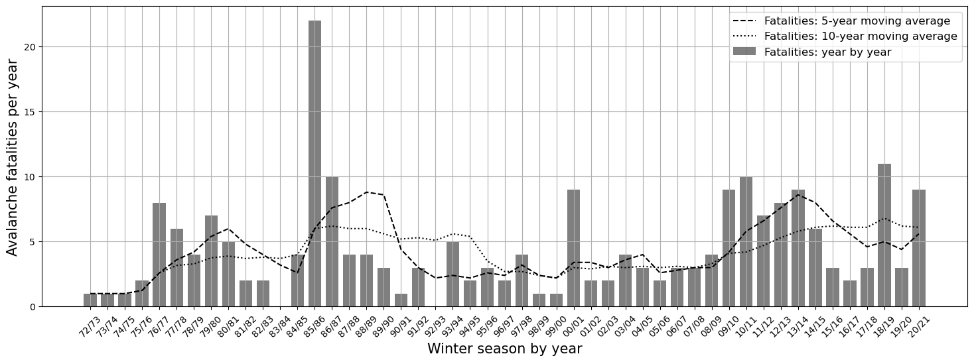
\includegraphics[width=\linewidth]{media/image1.png}
    \caption{Recreational avalanche fatalities in Norway by winter season from 1972 to 2021 with a 5 and 10-year moving average \parencites{NGI2019}{Varsom2021}.}
    \label{fig:rId8}

  \end{fullwidth}
\end{figure*}






While our focus is on backcountry travelers in avalanche terrain, the same issue is shared by many other outdoor recreation activities, including but not limited to hiking, mountain biking, paragliding, trail running, and white-water kayaking. The fatalities and respective hazard-causing deaths are documented in all of these cases. The number of hours backcountry travelers expose themselves to avalanches, also known as the base rate, is absent \parencites{Johnson2020}{Kahneman1973}. As such, a method to efficiently collect data on avalanche exposure is of value to the broader community of outdoor recreation.







Avalanches cause significant human and material losses \parencites{Schweizer2008}. Mitigation policies and prioritization require a qualitative basis from which to design strategies and allocate resources. \textcite{WMO2021} recommends a risk-based approach to warnings and mitigation (adopted by government agencies such as the Norwegian Water Resources and Energy Directorate) that requires base rate data. Due to the lack of exposure data, base rates are challenging to calculate in terms of people traveling in avalanche terrain. With base rate data, it is easier to understand which natural hazards need the most attention, the amounts of resources that are needed, and which measures are most efficient from a cost-benefit perspective.







The base rate information could also be used to validate whether an increase in objective danger correlates with avalanche danger levels. \textcite{Winkler2021} calculated a relative risk between the danger levels, but without a base rate, they could not calculate the absolute risk (i.e., micromorts). Furthermore, without a valid base rate measure, Bayesian approaches, which utilize diagnostic tests (also known as stability tests) to assess avalanche decision-making, lack important input data \parencites{Ebert2019}{Techel2020}.







Given the ubiquitous use of mobile phones in Norway \parencites{Statista2021}, with 99.9\% of the population having access to 4G coverage \parencites{MLGM2021}, there is a potential opportunity to obtain some insight into the total exposure to avalanche terrain. Telia, one of the largest mobile network operators (MNOs) in Norway, collects a vast amount of anonymized data through what is referred to as signaling data. Every time a phone communicates with a base transceiver station (BTS) (e.g., a phone call, text message, or the phone itself checks for new emails), signaling data is generated. On average, a Telia subscriber generates around 300-400 active and passive signaling events a day, or roughly 15 events per hour. The vast amount of data collected makes it an appealing data source when studying human mobility \parencites{Zhao2016}.







During the last few decades, telecom data have been widely used in the research community. Many useful findings of human activity have been reported for urban areas \parencites{González2008}{Song2010}. To our knowledge, there is no research applying telecom data in non-urban areas other than \textcite{Francisco2018}. The reason for this could be the relatively lower density of BTSs in rural and mountainous terrain, with the majority located where people live, work, and travel \parencites{Zhao2016}.







Norway has a vast number of remote mountains, fjords, and islands. It is also among the least densely populated countries globally, with a population density of 15 people per square kilometer \parencites{UN2021}. Despite this, the MNOs in Norway have been ranked among the top 10 providers worldwide with respect to cell phone coverage for several years in a row \parencites{Speedtest2021}. As a result of the excellent coverage, most mountainous areas in Norway have full 4G coverage \parencites{Telenor2021}{Telia2021}, and therefore their signaling data are expected to have some utility in these areas.







In this study, we attempted to use anonymized and aggregated signaling data to count how many people expose themselves to avalanche terrain around Tromsø, Norway. We selected this area as historically, nearly 2/3 of all recreational avalanche fatalities in Norway occur in this county \parencites{Varsom2021}. However, because no one has been able to accurately estimate how many people enter avalanche terrain in this region, it is impossible to say whether this high number of fatalities is solely due to more users in the area, or if it is more dangerous to ski in the area around Tromsø compared to the rest of the country. Without the base rate information, we are unable to determine which of the two hypotheses is correct \parencites{Johnson2020}{Kahneman1973}.







Secondly, we also want to use this method to help assess whether the fatal accident rate (FAR) from avalanches has increased or decreased during the last decade. Despite the number of avalanche fatalities over the last ten years having been relatively stable, there is a general agreement that there has been a significant increase in traffic amongst different groups of backcountry travelers in the same period. This view of increasing use is supported by a range of proxies, including the number of people seen in avalanche terrain, the number of vehicles at trailheads, and the sale of backcountry traveling equipment. This increase of use, combined with a relatively stable fatality count, suggests that the FAR has decreased during the last few decades \parencites{Techel2016}.







The challenges of determining the number of people exposing themselves to avalanche risk in the backcountry and calculating the risk of skiing in avalanche terrain, have been approached by several others using a range of imperfect methods. For example, \textcite{Zweifel2006} used light barriers and voluntary registration boards at four sites near Davos, Switzerland. Using these methods, \textcite{Zweifel2006} calculated the individual risk factor for this population and found it lower than the risk of driving a car. However, this was for very limited area of Switzerland, and represents an engaged and self-selecting audience that voluntarily provide registration information. There have also been several studies using GPS-tracking and surveys to assess terrain use \parencites{Buhler2016}{Hendrikx2014}{Hendrikx2016}{Sykes2020}{Thumlert2017}{Winkler2021}, but these studies are not representative for the whole population and are generally skewed towards more engaged and advanced users. Passive tracking of backcountry users with time-lapse camera technology has also been used \parencites{Saly2020}, but was also limited to a small geographic area. The use of telecom data for avalanche terrain is limited to a single study by \textcite{Francisco2018}, who undertook a case study to track backcountry users in the Sorteny valley, Andorra. They obtained access to raw call detail records (CDRs), including an estimated position for each record with an accuracy of 150 meters for a period of 20 days. From these CDRs, they created daily frequency plots and compared them with avalanche danger, temperature, wind, snow depth, solar radiation, and precipitation. Unfortunately, \textcite{Francisco2018} did not provide any information regarding how the position (latitude, longitude) was established or validated.



Our study attempted to build on these prior studies and used truly anonymized signaling data from Telia Company to count the total number of backcountry users within one avalanche forecasting zone in northern Norway. We also explored how these counts changed in relation to known drivers of usage, including weekends and holidays, and variable environmental conditions.







\section{Methods}



Telia uses telecom network data, which is one of the most extensive and continuously generated datasets in society today. The network data exceeds billions of data points every day in each Nordic country. These are stored in the Telia database for billing, network optimization, and other purposes. However, in contrast to regular data services, Telia can safeguard that no individuals can be identified in the dataset, while still providing extrapolated national movement patterns that are statistically representative for the entire population and not just Telia subscribers.







Using signaling data, Telia can produce mobility insights through a GDPR-compliant method. They do this by never storing, processing, or exposing data that can identify an individual, and the smallest result generated is in groups of 5 individuals within the same movement chain \parencites{Ågren2021}.







Telia does not have the exact position of each phone in their signaling data, and new data is only generated when the phone is actively or passively used (i.e., calling, SMS, transfer of data), but most smartphones today are constantly checking for updates, and thus constantly generating signaling data.







Each signaling data record includes a timestamp and the coverage area (Cell ID) to which the phone is connected. The best server estimate (BSE), which is the estimated coverage area, is defined for each Cell ID. Most BTSs have several Cell IDs due to the different antennas pointing in diverging directions. Thus, the Cell ID provides more specific information about the position of the phone than only using the BTS. The BSE consists of uniquely shaped polygons representing the coverage area of each Cell ID. The MNOs collect a lot of data, but the utility of that data for research purposes is limited due to privacy concerns. Telia Company does not use any triangulation methodology to define a more exact location due to their strict privacy policy, but by analyzing the data over time, it is possible to generate movement chains from the signaling data. Telia’s algorithms process the movement chains to form insights. They were originally intended for urban areas, but we have employed them to assess whether we can count skiers’ phones in avalanche terrain using the insights from signaling data.







The algorithms that process the movement chains are designed to capture three different patterns. The overview below intends to provide a working understanding of how Telia distill relevant data for each report.





\begin{enumerate}


  \item Activity report – where crowds are spending time without directional movement.



  \item Routing report – where crowds are passing by without stopping.



  \item Origin-destination report – the trips made by crowds between origins and destinations.


\end{enumerate}





In this study, we utilize the activity report, which captures how many subscribers spend a defined amount of time in a defined geographical area. The activity report can be produced from a regional level and down to a statistical grid, with the lowest resolutions being 500 x 500 meters in a dense urban area. The resolution is flexible, so the grids are larger to secure GDPR compliance in rural settings. It is possible to filter the amount of time spent in a defined area, or use timestamps to reveal when visitors arrived or left an area during the day.







The spatial resolution of mobile network data is dependent on the size of the Cell ID that the cellphone has been communicating with. Each BTS has several Cell IDs with a geographic coverage area. When a device moves around it will connect to multiple different Cell IDs, leaving a movement chain. The initial processing involves turning this raw data trace into dwells (activities taking place in one location) and movements (Figure 2).



\begin{figure*}[h]
  \begin{fullwidth}


    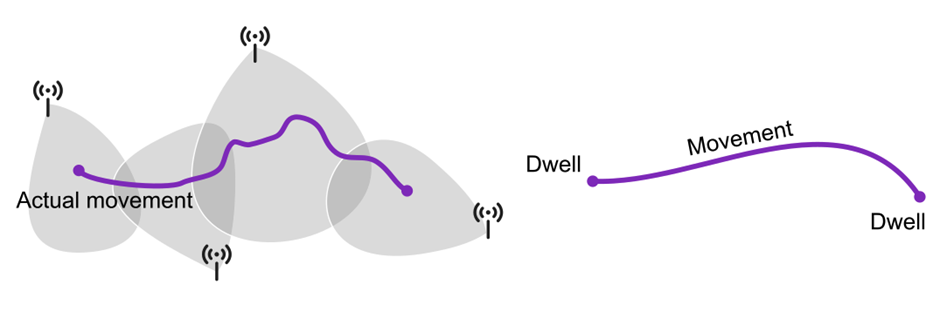
\includegraphics[width=\linewidth]{media/image2.png}
    \caption{The movement of each cellphone could be tracked through different coverage areas.}
    \label{fig:rId9}

  \end{fullwidth}
\end{figure*}






To utilize this methodology, we defined a geographical area for the avalanche terrain. We also defined where people live (i.e., populated areas) to identify areas that we could distinguish between avalanche terrain and populated areas. We defined populated areas and avalanche terrain on a map using GIS software (Figure 3). Definitions and methods for defining these areas are outlined in the sections below.



\begin{figure}
  \begin{fullwidth}
    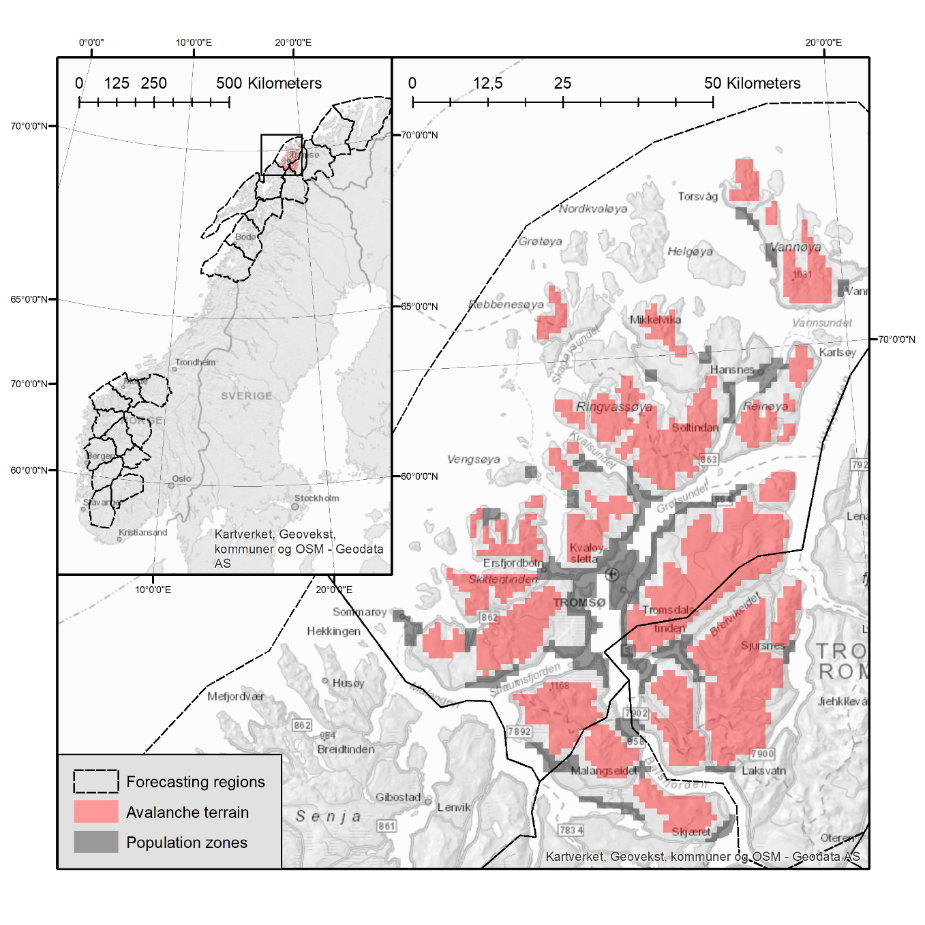
\includegraphics[width=\linewidth]{media/image3.png}
    \caption{The case study area Tromsø, Northern Norway. Avalanche terrain is colored in red, while the populated areas are colored in dark gray. The avalanche forecast regions are delineated using a dashed line on the inset map.}
    \label{fig:rId10}

  \end{fullwidth}
\end{figure}






\subsection{Populated areas}



\textcite{StatisticsNorway2021} has created a GIS layer with the number of inhabitants per 1x1 square kilometers. We used this layer and defined populated areas as grid cells with more than ten inhabitants.







\subsection{Avalanche terrain}



Avalanche terrain can be defined using the Avalanche Terrain Exposure Scale (ATES) framework \parencites{Statham2006}. Using the nationwide ATES layer developed by Larsen et al.(2020), we defined avalanche terrain as the sum of simple, challenging, and complex avalanche terrain. Numerous houses and roads lie within avalanche terrain \parencites{Kalsnes2021}. We removed all avalanche terrain within 300 meters of a house or a road from the GIS layer. The distance of 300 meters was chosen to avoid counting people that are driving a car or living in a house, but not moving between a populated area and avalanche terrain.







\subsection{Mobility analysis}



The two layers with populated areas and avalanche terrain were exported and shared with Telia. They applied the layers with their BSE of the coverage area and identified areas where it was possible to distinguish between populated regions (purple) and potential avalanche terrain (red) (Figure 4). Using the insights from the movement chains, Telia counted how many phones traveled into avalanche terrain using signaling data.







Given the nature of the terrain, the most common backcountry trips around Tromsø include a vertical elevation gain of between 800-1200 vertical meters. Assuming a regular uphill pace of 400-600 vertical meters per hour, this could cause uphill travel to take as few as 2 hours for the fittest recreationists. Most people also hike and ride during the daytime. Therefore, we added a filter that only kept phones that were in avalanche-prone terrain for at least 2 hours between 07.00-23.00, during the 2019-2020 avalanche forecasting season (1\textsuperscript{st} of December until 31\textsuperscript{st} of May). This period includes the spring season when the Covid-19 pandemic started. Large parts of Norway closed down on March 13\textsuperscript{th} and there is likely a drop in tourists after this date.






\subsection{Validation}



To improve the insights from the movement chains, Telia has developed an algorithm that can assign the most likely position within the Cell ID. Telia has targeted the algorithm against normal behavior, which means that the positions will be biased towards populated areas and roads where most people travel. The in-depth details regarding the algorithm are considered a trade secret and are not disclosed due to Telia's commercial interests. Using the output from the algorithm enables us to compare the GPS position to signal data-derived position. The GPS on their watch has a position accuracy of 5-10 m \parencites{Wing2005}.




\begin{figure*}[t]
  \begin{fullwidth}



    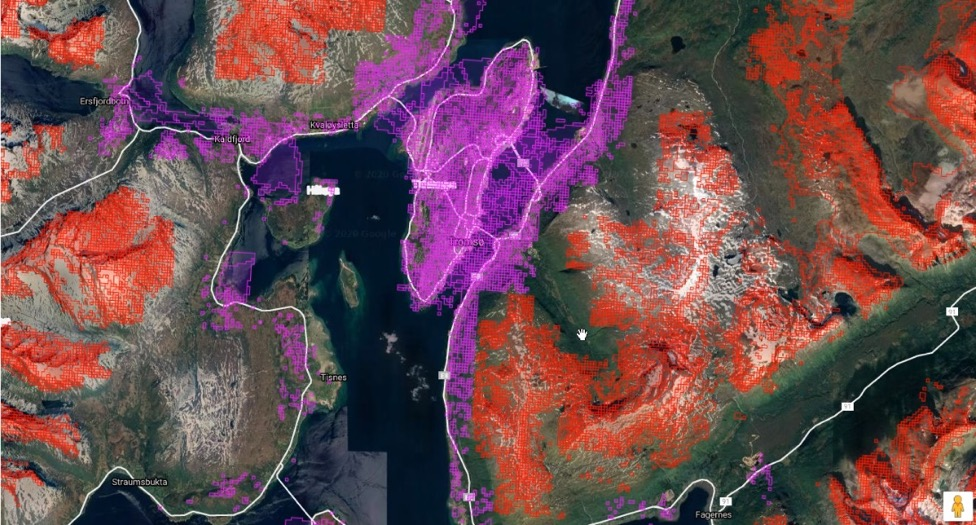
\includegraphics[width=\linewidth]{media/image4.jpg}
    \caption{Example of identified areas around Tromsø where the Telia could distinguish between populated areas (purple) and potential avalanche terrain (red) given their BTS coverage in the region.}
    \label{fig:rId11}

  \end{fullwidth}
\end{figure*}


\subsection{Correlation with other usage factors }



We correlated the number of people per day against the amount of daylight, number of avalanche bulletin page views, weekends and holidays, the daily avalanche danger, percentage of cloud cover, wind strength, and precipitation. All weather parameters were aggregated between 07.00 in the morning and 23.00 in the evening to only account for the conditions during daytime. Amount of daylight was calculated for a latitude of 69° North \parencites{SatAgro2019}. The daily avalanche danger level was provided by \textcite{Varsom2021} and the number of page views for the avalanche forecast on Varsom.no was provided by Google Analytics. Weekends and holidays were encoded as binary values of 0 or 1, with weekends and holidays coded as 1 and weekdays coded as 0. The weather variables were downloaded from the \textcites{NorwegianCentreforClimateServices2021} on an hourly basis.



\begin{table}
  \begin{fullwidth}
    \caption{Number of people in potential avalanche terrain versus different variables that could be controlling number of people in avalanche terrain. * Variable is not significant.}

    \centering
    \begin{tabular}{@{} l l l  @{}}
      \toprule
      \textbf{Number of people per day versus:} &
      \textbf{R}{\textsuperscript{\textbf{2}}}
                                                & \textbf{p-value}   \\
      \midrule

      Amount of daylight                        & 0.186            &
      < 0.01                                                         \\

      Weekend and holidays                      & 0.073            &
      < 0.01                                                         \\

      Avalanche forecast page views             & 0.045            &
      < 0.01                                                         \\

      Avalanche bulletin                        & 0.007            &
      0.244*                                                         \\

      Cloud cover                               & 0.004            &
      0.374*                                                         \\

      Wind strength                             & 0.002            &
      0.521*                                                         \\

      Precipitation                             & 0.000            &
      0.917*                                                         \\
      \bottomrule
    \end{tabular}
  \end{fullwidth}
\end{table}


\begin{table*}[t]
  \begin{fullwidth}

    \centering
    \caption{Minimum, maximum, median, and 95\% of all point distances between GPS track and signaling data spatial locations.}
    \begin{tabular}{@{} l r r r r r @{}}
      \toprule
                                     & \textbf{Min} & \textbf{Max} &
      \textbf{Median}                &
      \textbf{95\% of points within} &
      \textbf{N (samples)}                                           \\
      \midrule

      Trip 1                         & 455 m        & 8,216 m      &
      4,188 m                        & 7,580 m      & 74             \\

      Trip 2                         & 7,876 m      & 21,502 m     &
      13,607 m                       & 20,424 m     & 93             \\

      Trip 3                         & 19 m         & 16,213 m     &
      2,596 m                        & 14,212 m     & 135            \\

      Trip 4                         & 1,997 m      & 8,919 m      &
      6,911 m                        & 8,736 m      & 114            \\

      All trips                      & 19 m         & 21,502 m     &
      6,523 m                        & 12,920 m     & 416            \\
      \bottomrule
    \end{tabular}
  \end{fullwidth}
\end{table*}



\section{Results}



\subsection{Mobility analysis}



Using the mobility analysis methods, we estimated that 13,666 people were in avalanche terrain for at least two hours during the 2019-2020 season (December 1\textsuperscript{st}, 2019, to May 31\textsuperscript{st}, 2020, consisting of 182 days). The number of people in avalanche terrain per day varied from 0 to 118, with an average of 75 people per day.






Amount of daylight had the strongest, albeit very low, correlation (\emph{R}\textsuperscript{2} = 0.186, \emph{p} < 0.01), followed by weekends and holidays (\emph{R}\textsuperscript{2} = 0.073, \emph{p} < 0.01) and the number of forecast page views (\emph{R}\textsuperscript{2} = 0.045, \emph{p} < 0.01). We also correlated against precipitation, wind, daily avalanche danger and cloud cover, but none of these parameters were statistically significant (Table 1).













\subsection{Positional Validation}



Using a phone with a special SIM card that was whitelisted (i.e., not anonymized in the telecom network—users gave specific consent for this), our validation focused on the positional accuracy of the signaling data relative to the synchronous GPS records. When we compared these, we discovered that there was a discrepancy between the two data sets. In the examples (Figure 5), we can see that the estimated positions from the signaling data does not resemble the GPS track. Most of the signaling data positions are estimated to be in the valley bottom, following road corridors or out on the fjords. For all four trips, the positional difference ranged from 19 meters to 21,502 meters. The median positional difference was 6,523 meters and 95\% of the points were within 12,920 meters (Table 2).









\begin{figure*}[b]
  \begin{fullwidth}



    \centering
    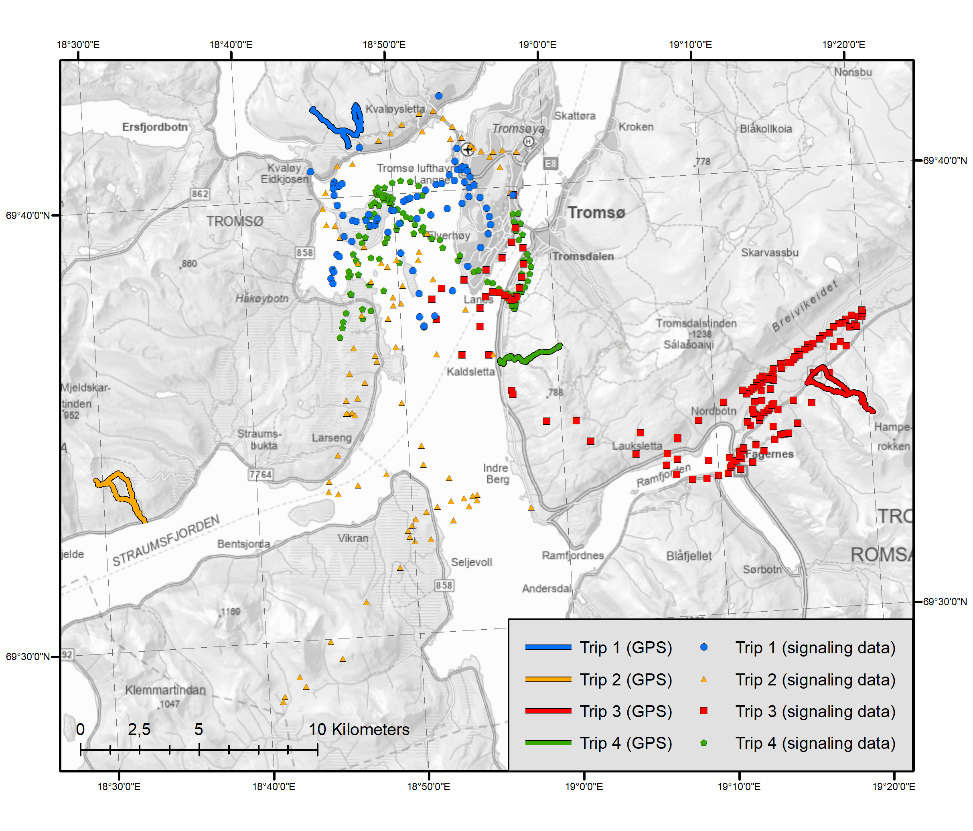
\includegraphics[width=.9\linewidth]{media/image5.png}
    \caption{Comparison of 4 different color-coded trips using GPS data (line) and estimated positions from the signaling data (circle, triangle, square and pentagon).}
    \label{fig:rId12}

  \end{fullwidth}
\end{figure*}





\section{Discussion}



A qualitative review of the four GPS tracks and the signaling data estimated locations shows discrepancies in the estimated positions from the two data sets as shown in Figure 4. This is further supported by our quantitative analysis, where all trips were off by several hundred meters to several kilometers (Table 2). Clearly these positional results are disappointing, and in strong contrast to the reported 150-meter accuracy of the geolocation in mountainous terrain in Andorra \parencites{Francisco2018}. It is difficult to directly compare our results regarding accuracy given that we do not know how Francisco et al. estimated their positional data, or how they validated the accuracy of the signaling data. The differences could be due to several factors, including the potential lower density of BTSs in Troms and/or the algorithm in Norway being designed by Telia for use in urban areas. By comparison, \textcite{Jansen2021} found the position accuracy of telecom data to be roughly 500 meters in the cities and 3,000 meters in rural areas.







To validate our data, we wanted to check whether the Telia’s algorithm estimated the correct locations in rural areas where the coverage areas for each Cell ID are much larger. The algorithm is tuned to work in populated areas where the coverage areas for each Cell ID are small, which makes it easier to estimate the position moving through different coverage areas. The difference in density of BTSs was one of the significant uncertainties in our study. After sending mountain runners out with whitelisted phones, we learned that the positioning of each phone did not work as well as we had initially hoped. When whitelisted phones were compared with actual GPS tracks, we found that the signaling data-derived locations would follow the road corridors leading to the mountains. When our mountain runners parked their cars at the foot of the mountain and started running up, the estimated position stayed in the valley bottom or out on the fjords. We quickly learned that what we initially believed to be a good dataset of ski traffic in the region from the signaling data was biased by the large coverage area of each Cell ID outside the cities. We think there are two primary reasons for this:





\begin{enumerate}


  \item Telia’s algorithm is targeted using data from people travelling on roads between houses, work, stores, etc.



  \item
        The coverage area outside the populated areas is too large to define whether people are up in the mountains or not.


\end{enumerate}





In the bigger picture, these problems are not that surprising. Mobile networks are built and optimized for urban areas where most people live, work and travel. Telecom companies specifically design and build their networks to cover large areas with the fewest possible number of antennas. We are trying to achieve the opposite, capturing signaling data from unpopulated areas where people usually do not travel due to lack of infrastructure. In a broader sense, this is the main limitation of our ability to accurately estimate the position of each phone in rural areas.







We also compared the data with parameters we expected would affect the number of people out in the mountains to initially verify our data. The parameters were amount of daylight (expected positive correlation), number of bulletin page views (expected positive correlation), the occurrence of weekends and holidays (expected positive correlation), rain (expected negative correlation), cloud cover (expected negative correlation), wind strength (expected negative correlation), and avalanche danger (expected negative correlation). For weather data, we only investigated data between 07.00-23.00 because this was the period, we counted people and would likely affect the decision to go skiing or not. The most important coefficient was amount of daylight, followed by weekend/holidays and number of bulletin page views. The various weather parameters were not significant and had very low coefficient scores. The results are logical because most backcountry travelers are outside when there is daylight in the Arctic, but we had hoped for a better fit towards the weather parameters. This lack of fit in our simple correlations is most likely due to the inaccurate location positions from the signaling data, resulting in the additional counts of users that were not in avalanche terrain, but were included in our data set. This resulting data set is therefore much noisier and includes people in other areas outside of the immediate populated areas, but not necessarily in avalanche terrain.




\begin{originalPurpose}

  The objective of this manuscript is to document our attempts to use signaling data from telecom networks to count the number of backcountry travelers in avalanche terrain within the Tromsø avalanche forecasting region in Northern Norway. If this method had permitted an accurate count of people in avalanche terrain, we would have been able to obtain a very representative sample of overall terrain usage. Combined with the observed number of fatalities in the same avalanche forecasting region, we would also have been able to calculate how risky the activity is in terms of micromorts. Furthermore, we could have tracked terrain usage over several winter seasons to obtain data to assess whether there are any trends concerning the number of people accessing avalanche terrain over time and whether increased interventions, including the uptake of avalanche awareness courses and improved avalanche forecasting, is evident in a change in micromorts over time. To our knowledge, there have not been any studies utilizing telecom network data in non-urban areas. We believe that our results are significant for a broader audience to showcase potential pitfalls when using this type of data. We also highlight the importance of validating this type of data.




\end{originalPurpose}





\newpage
\section{Limitations}



As already noted in our discussion above, the positional accuracy of the signaling data when compared to the GPS data is the main limitation to the use of this methodology as currently presented. Access to the raw data, prior to analysis by the algorithm, which is targeted for urban use, might alleviate some of these issues, but this was considered outside the scope of the current study.







Furthermore, the reliability of any mobile phone tracking in avalanche terrain depends on users leaving their phone turned on for the duration of their trip. Many backcountry travelers elect to turn their cell phones off to purposefully save battery power for emergency calls. Travelers are also generally encouraged to turn their cell phones off or to flight mode to prevent potential interference with avalanche transceivers. This reality was reflected in a winter backcountry survey by \textcite{Ortega2018} in Alaska, which showed that of the 63 users interviewed, approximately half of them typically leave their phone turned on whereas the rest turn theirs off or to flight mode.







The main limitation in making telecom data viable for counting people in avalanche-prone terrain is the lack of numerous BTSs in mountainous areas. A more specific algorithm could improve the data quality for this use case, but the BTS density is likely the key factor that would make the method more viable if a mountainous area with a higher density of BTSs is found.





\section{Conclusion}



In urban areas, each BTS with several Cell IDs is close together, which means that Telia can estimate more accurate positions given the small coverage area for each Cell ID. Even though Norway has exceptional cellphone coverage compared to many other countries, it is still insufficiently dense in our non-urban and mountainous study area case study. The long distances between the BTSs, and therefore large coverage areas, combined with the populated area-targeted algorithm, are the most likely reasons for the inability to accurately calculate the position of each phone in avalanche terrain. The poor correlation between the GPS track and the position of the whitelisted phones means that we cannot trust the positional accuracy of this initial dataset as provided by Telia. Future work should focus on making a model that is independent of where most people travel. This study provides a useful, yet unsuccessful, case study that demonstrates the limits of signaling data for use in non-urban mountainous areas. It has relevant implications for the application of signaling data tracking to other outdoor recreation activities. We highlight the importance of validating positional data from signaling data to be used in mobility studies in remote areas.




\section{Data}

The data that support the findings of this study are available at \url{https://zenodo.org/record/7891581}.


\section{Funding}
This work is financially supported by the Norwegian Water Resources and Energy Directorate and Telia Company, who have generously provided dedicated working hours for the project.

\section{Conflict of interest}
The authors declare that they have no conflict of interest.


\printbibliography
\end{document}